% !TEX encoding = UTF-8 Unicode

\documentclass[12pt,a4j,titlepage]{ltjsarticle}
\usepackage{semi}
\usepackage{here}

% \title{}
% \author{}
% \date{}

\begin{document}

\begin{titlepage}
  \begin{center}
  
    \vspace*{20truept}
    
    {\LARGE 2022年度 卒業論文}
    
    \vspace*{75truept}
    
    {\Huge 初学者向けネットワーク通信の学習を} %論文タイトル

    \vspace{10truept}

    {\Huge 支援するシミュレータWeb教材 } %論文タイトル 長い場合 改行1

    \vspace{10truept}

    {\Huge } %論文タイトル 改行2

    \vspace{85truept}
    
    {\LARGE 指導教員 須田 宇宙 准教授}
    
    \vspace{60truept}
    
    {\LARGE 千葉工業大学 情報ネットワーク学科}
    
    \vspace{15truept}
    
    {\LARGE 須田研究室}
    
    \vspace{70truept}
    
    {\LARGE 1932047 氏名 小松崎 嵩史 } % 氏名は消さない 学生番号 氏名 名前

    \vspace{70truept}
    
  \end{center}
  \begin{flushright}

    {\LARGE 提出日 2023年1月17日}
  
  \end{flushright}
\end{titlepage}
\setcounter{page}{0}\pagenumbering{roman}\pagestyle{plain}
\tableofcontents
% 表目次
\listoftables
% 図目次
\listoffigures

\clearpage
\setcounter{page}{0}\pagenumbering{arabic}
\section{緒言}%<1章>

%背景
DX(Digital Transformation)の実現に向けて,IT人材の確保・育成は一番大きな課題となっている.
IT人材の確保・育成を促進するため,2020年より小学校プログラミング教育から始まる情報教育の推進が図られている.
2022年より,高等学校においても新しい学習指導要領が改訂され,「情報Ⅰ」が共通必履修科目となっている.
また,大学入学共通テストにおいて2025年1月より,「情報Ⅰ」が出題範囲の「情報」が新教科として出題される予定となっている.

%問題点
情報教育の学習内容において,ネットワークの学習はプログラミングに比べて,講義形式の授業が多くなる点が問題点として挙げられる.
実習形式での授業が難しい理由として,学習指導要領でプログラミングを実習形式で学ぶことが勧められていること,ネットワークの実習を行うために,通信機器,仮想環境などの準備が難しいことが考えられる.
紙面の文字や図を基にした講義形式の授業では,初学者がネットワーク通信の層の動きや違いを理解することは難しいと考えられる.

%目的
これらの問題に対して,生徒や学生に配布されるタブレットや,小型のPCで利用できるWeb教材を講義形式の授業の補助に利用することで,問題点の改善に繋がると考えた.
そこで,本研究では上記のWeb教材を作成することを目的とする.
\clearpage

\section{DXについて}%<2章>
\subsection{概要}
DXとは,Digital Transformationの略称である.
企業がグローバル環境の激しい変化に対応し,データとデジタル技術を活用して,顧客や社会のニーズを基に,製品やサービス,ビジネスモデルを変革することである.
また,業務そのものだけでなく,組織,企業文化・風土を変革し,持続的な企業価値の向上を図ることである\cite{dx_gaiyou}. 

\subsection{DX推進の課題}
国内外の企業に向けた調査内にある,デジタル化を進める上での課題や障壁の日本企業(n=1296)の解答を抜き出したグラフを下の図\ref{fig:dx}に示す\cite{dx_kadai}.
デジタル化を進める上での課題や障壁として,人材不足が67.6\%と最も多く,次にデジタル技術の知識・リテラシー不足が44.8\%となっている.
IT人材の不足の解決には,社内人材の育成やアウトソーシングといった方法が考えられるが,持続的な企業価値の向上を図るためには,将来にわたって情報教育の推進が必要だと考えられる.
\\
\begin{figure}[h]
\centering
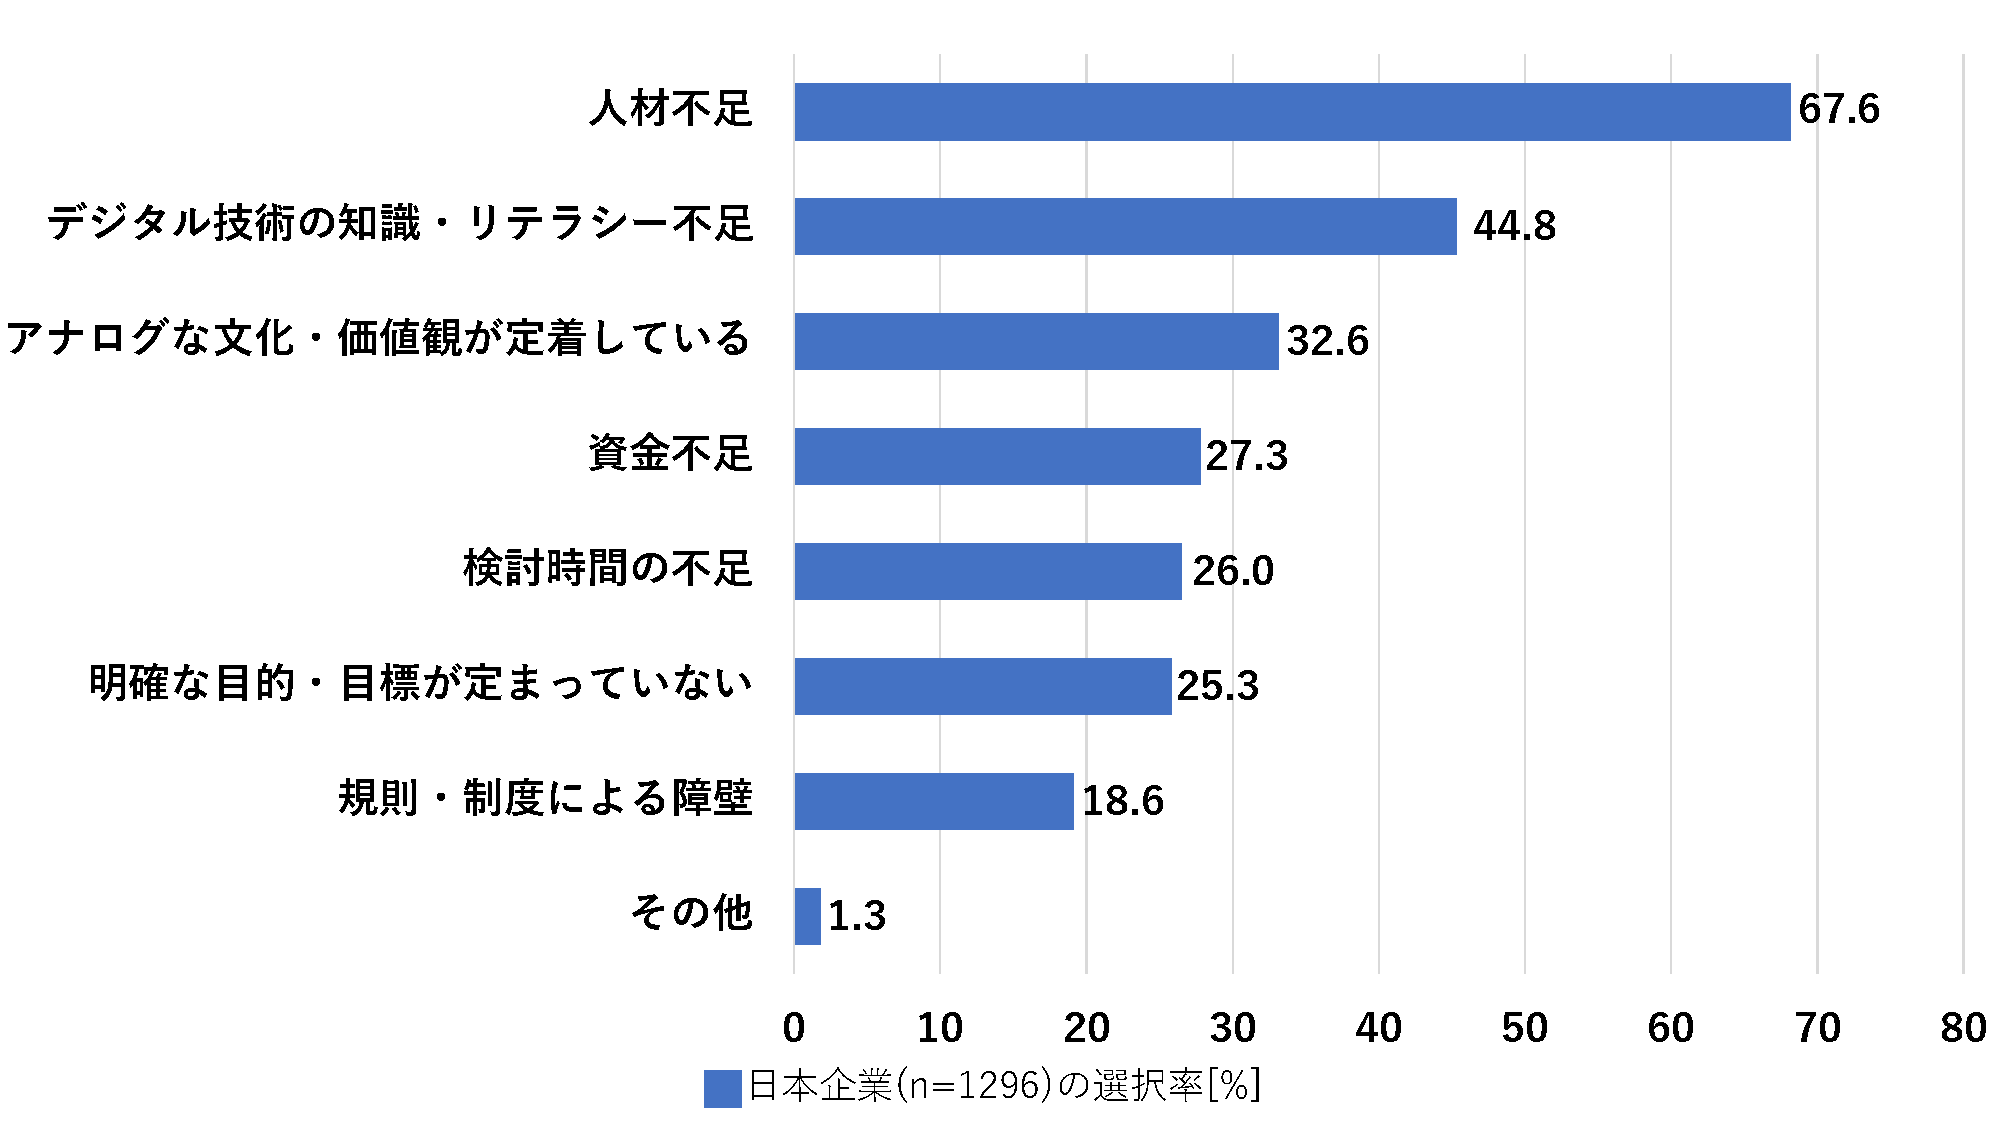
\includegraphics[clip,width=110mm]{figures/dx.pdf}
\caption[デジタル化を進める上での課題や障壁]{デジタル化を進める上での課題や障壁(複数選択)\linebreak}
\label{fig:dx}
\end{figure}

\clearpage

\section{情報教育について}%<3章>
\subsection{概要}
情報教育とは,子どもたちの情報活用能力の育成を図るものである.情報活用能力とは,「情報及び情報手段を主体的に選択し,活用していくための個人の基礎的な力」である.
情報教育の目標は以下の3つの観点に整理される\cite{kyoiku_gaiyou}.

\begin{enumerate}

\item[1] 情報活用の実践力\mbox{}\\
課題や目的に応じて情報手段を適切に活用すること\\
必要な情報を主体的に収集,判断,表現,処理,創造し,受け手の状況などを踏まえて発信,伝達できる能力

\item[2] 情報の科学的な理解\mbox{}\\
情報活用の基礎となる情報手段の特性の理解\\
情報を適切に扱うこと,自らの情報活用を評価,改善するための基礎的な理論や方法の理解

\item[3] 情報社会に参画する態度\mbox{}\\
社会生活の中で,情報や情報技術が果たしている役割や及ぼしている影響を理解し,情報モラルの必要性や情報に対する責任について考え,望ましい情報社会の創造に参画しようとする態度

\end{enumerate}
上記の目標を達成するために,情報活⽤能⼒を⾔語能⼒と同様に学習の基盤となる資質・能⼒と位置付け,小学校,中学校,高等学校と段階的に学習していく.

\subsection{小学校プログラミング教育}
\subsubsection{概要}
コンピュータ等を活用することが求められるこれからの社会では,コンピュータを理解し,活用していく力を身に付けることは,どのような職業に就くとしても極めて重要である.
そこで,導入されたのが小学校プログラミング教育である\cite{syogaku_pro}.

小学校プログラミング教育は,学習指導要領において「学習の基盤となる資質・能力」と位置付けられた「情報活用能力」の育成や情報手段(ICT)を「適切に活用した学習活動の充実」を進める中に,適切に位置付けられる必要がある.
よって,小学校プログラミング教育のねらいは情報教育の目標3つに対応した以下の3つに整理される.
\begin{enumerate}

\item[①] プログラミング的思考を育む\mbox{}\\
プログラミング的思考とは,自分が意図する活動を実現するためにどのような動きの組み合わせが必要であり、一つ一つの動きの組合わせをどのように改善していくべきかなどを論理的に考えていく力のことである.

\item[➁] 身近な生活でコンピュータが活用されていること,問題解決に必要な手順があることに気づく\mbox{}\\
コンピュータはプログラムで動いていることや,コンピュータに意図した処理を行わせるためには手順が必要なことなどの「気づき」が重要である.
そして,「気づき」をもとにコンピュータをより良い人生や社会を築くことといった,主体的に取り組む態度を涵養する.

\item[③] 各教科等の中で実施する場合については,「教科等での学びをより確実なものにする」こと\mbox{}\\
小学校プログラミング教育は,新しい教科としてではなく既存の授業の中でプログラミングを学んでいく.
学習指導要領に例示されているものとして,小学校5年生の算数の多角形や,小学校6年生の理科の電流がつくる磁力などの単元でビジュアル言語を利用したプログラミングによって,法則や仕組みを体験的に学習することが出来る.

\end{enumerate}
\subsubsection{小学校プログラミング教育におけるネットワーク通信の学習内容}
情報教育は,小学校,中学校,高等学校と段階的に行われる.一番最初である小学校プログラミング教育は,コンピュータに慣れ親しませるという段階から始まる.
また,小学校プログラミング教育は


\subsection{中学校技術・家庭科(技術分野)内容「D 情報の技術」}
\subsubsection{概要}
\subsubsection{中学校技術・家庭科におけるネットワーク通信の学習内容}

\subsection{高校「情報Ⅰ」}
\subsubsection{概要}
\subsubsection{高校「情報Ⅰ」におけるネットワーク通信の学習内容}

\subsection{ネットワークの学習教材について}
\subsubsection{「情報Ⅰ」教科書付属のシミュレータ}
\subsubsection{「情報Ⅰ」動画教材}

\clearpage

\section{ネットワークの基礎知識}%<4章>

\subsection{OSI}
\subsubsection{概要}
\subsubsection{OSI参照モデル}
\subsection{TCP/IP}
\subsubsection{概要}
\subsubsection{データリンク層}
\subsubsection{インターネット層}

\subsubsection{Ethernetフレーム}
\begin{figure}[h]
\centering
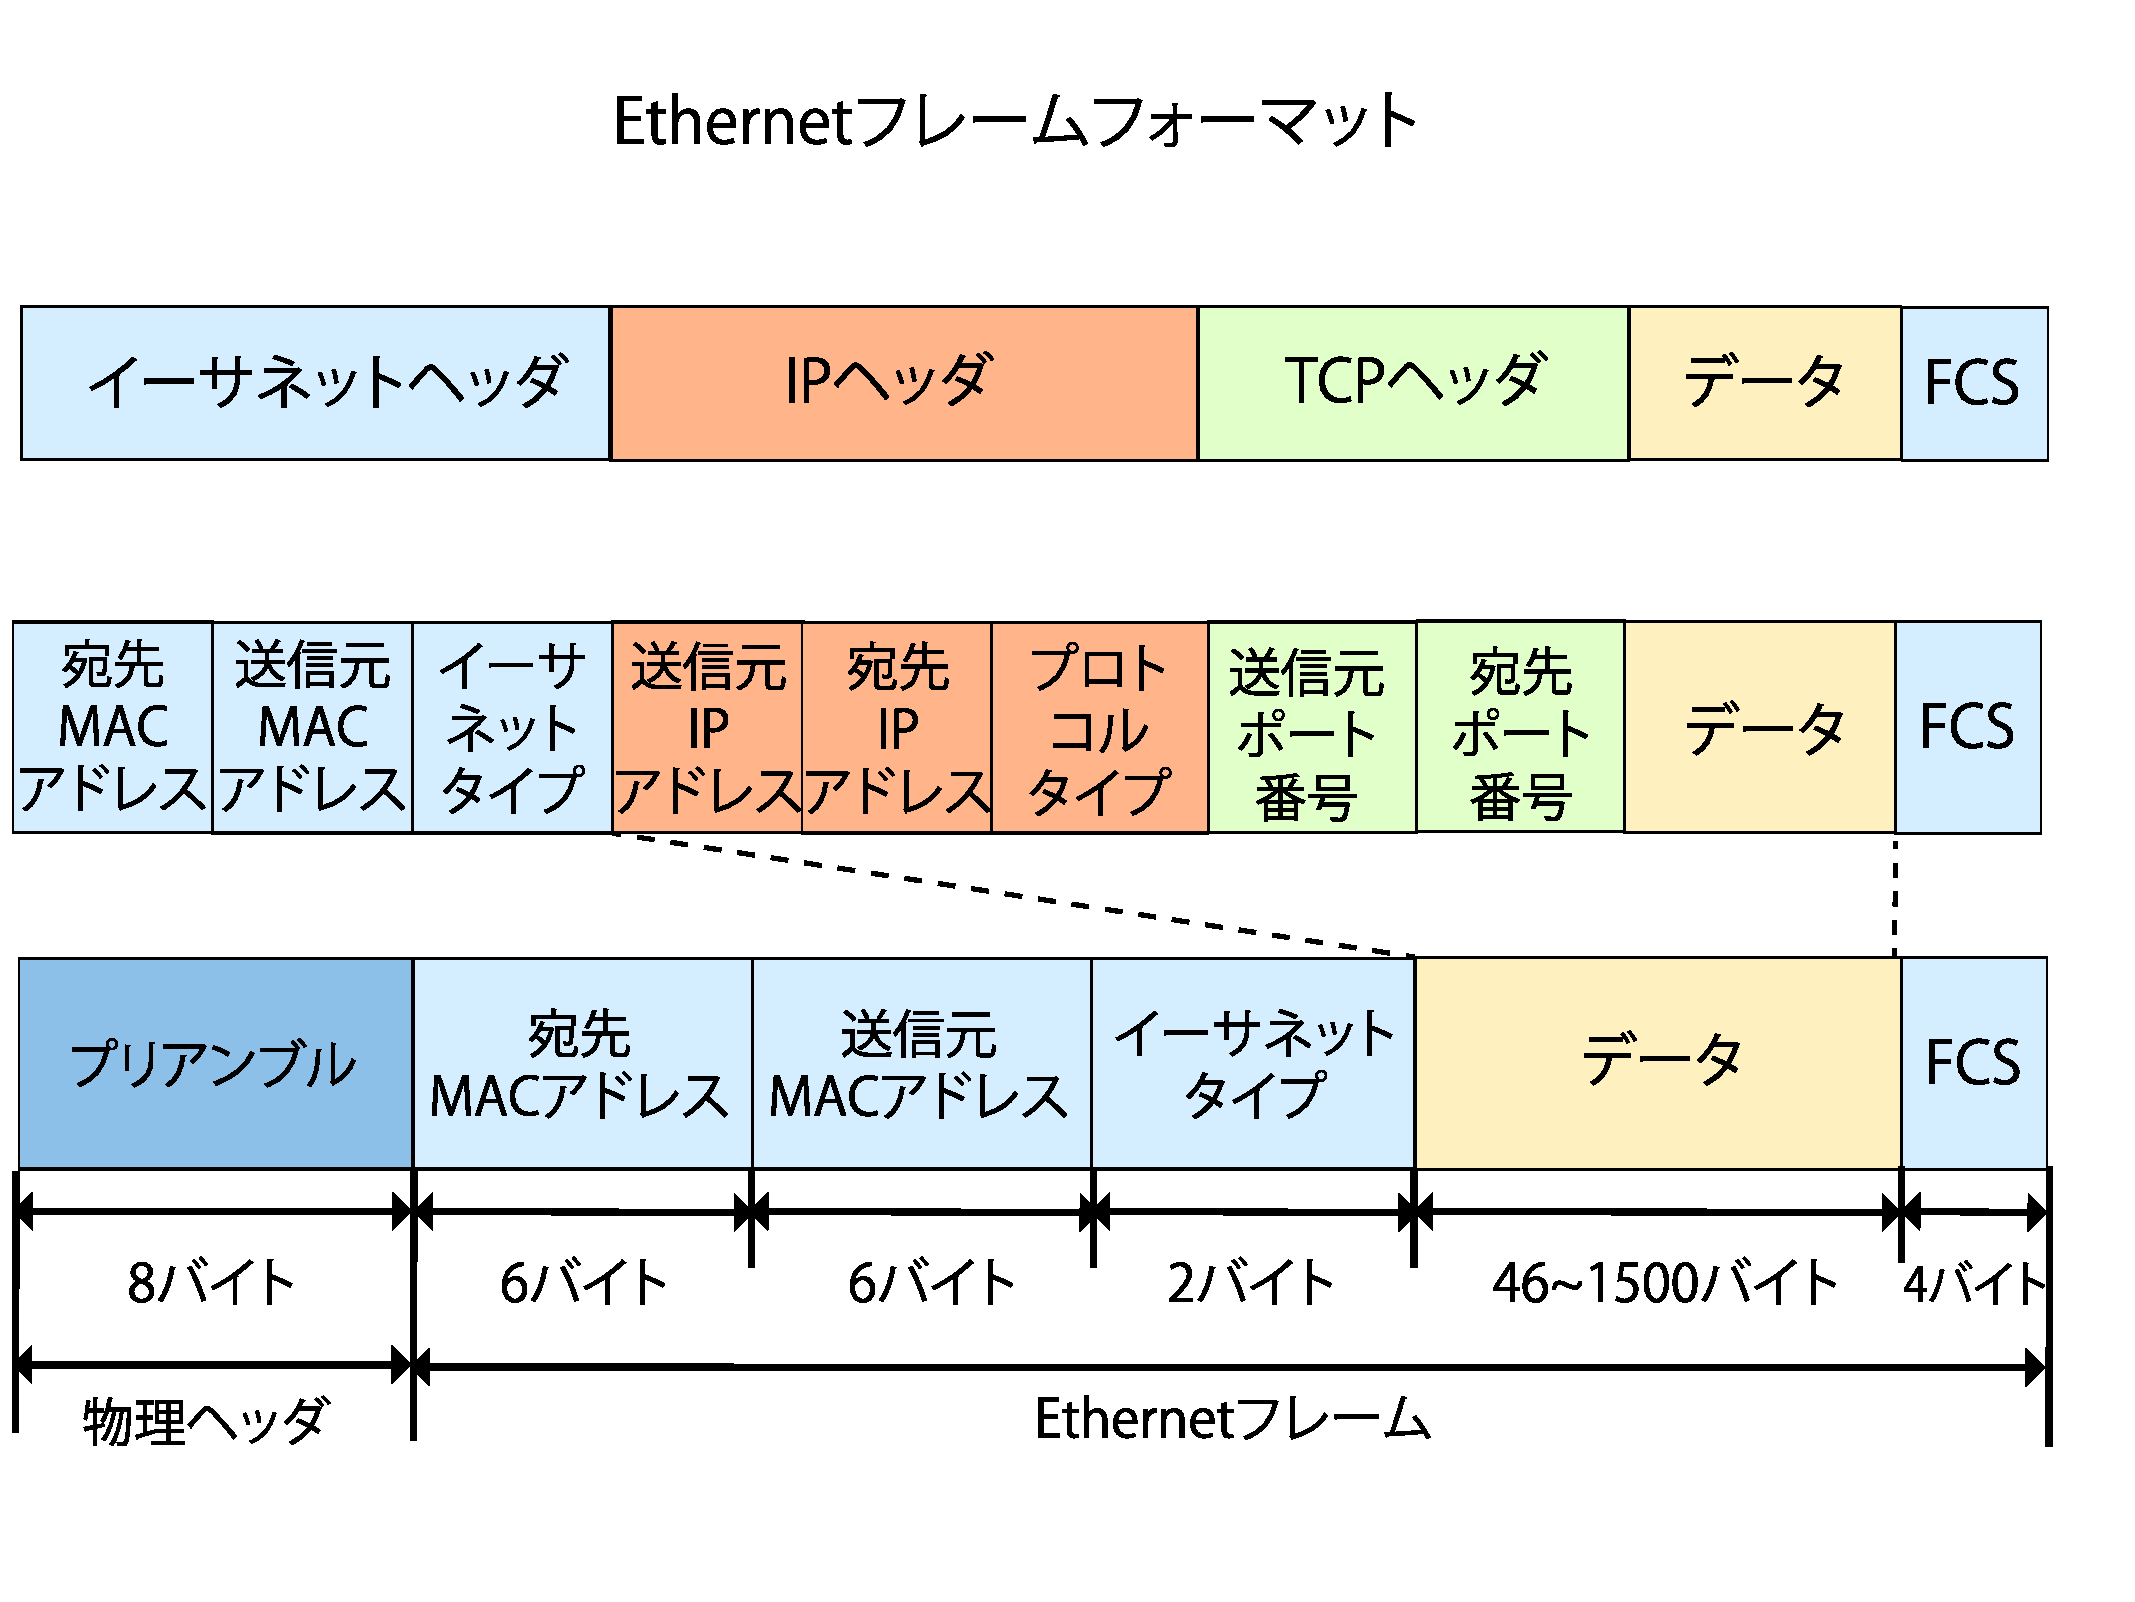
\includegraphics[clip,width=85mm]{figures/ethernet.pdf}
\caption[Ethernetフレームの概略図]{Ethernetフレームの概略図\linebreak}
\label{fig:ether}
\end{figure}

\subsubsection{IPアドレス}
\subsubsection{MACアドレス}

\clearpage

\section{開発する教材のコンセプト}%<5章>
a
\subsection{学習目的}
\subsection{教材の利用環境}
\subsection{教材の学習内容}
\subsection{教材の画面設計}

\clearpage

\section{教材の画面構成}%<6章>
\subsection{概要}

\begin{figure}[h]
\begin{center}
 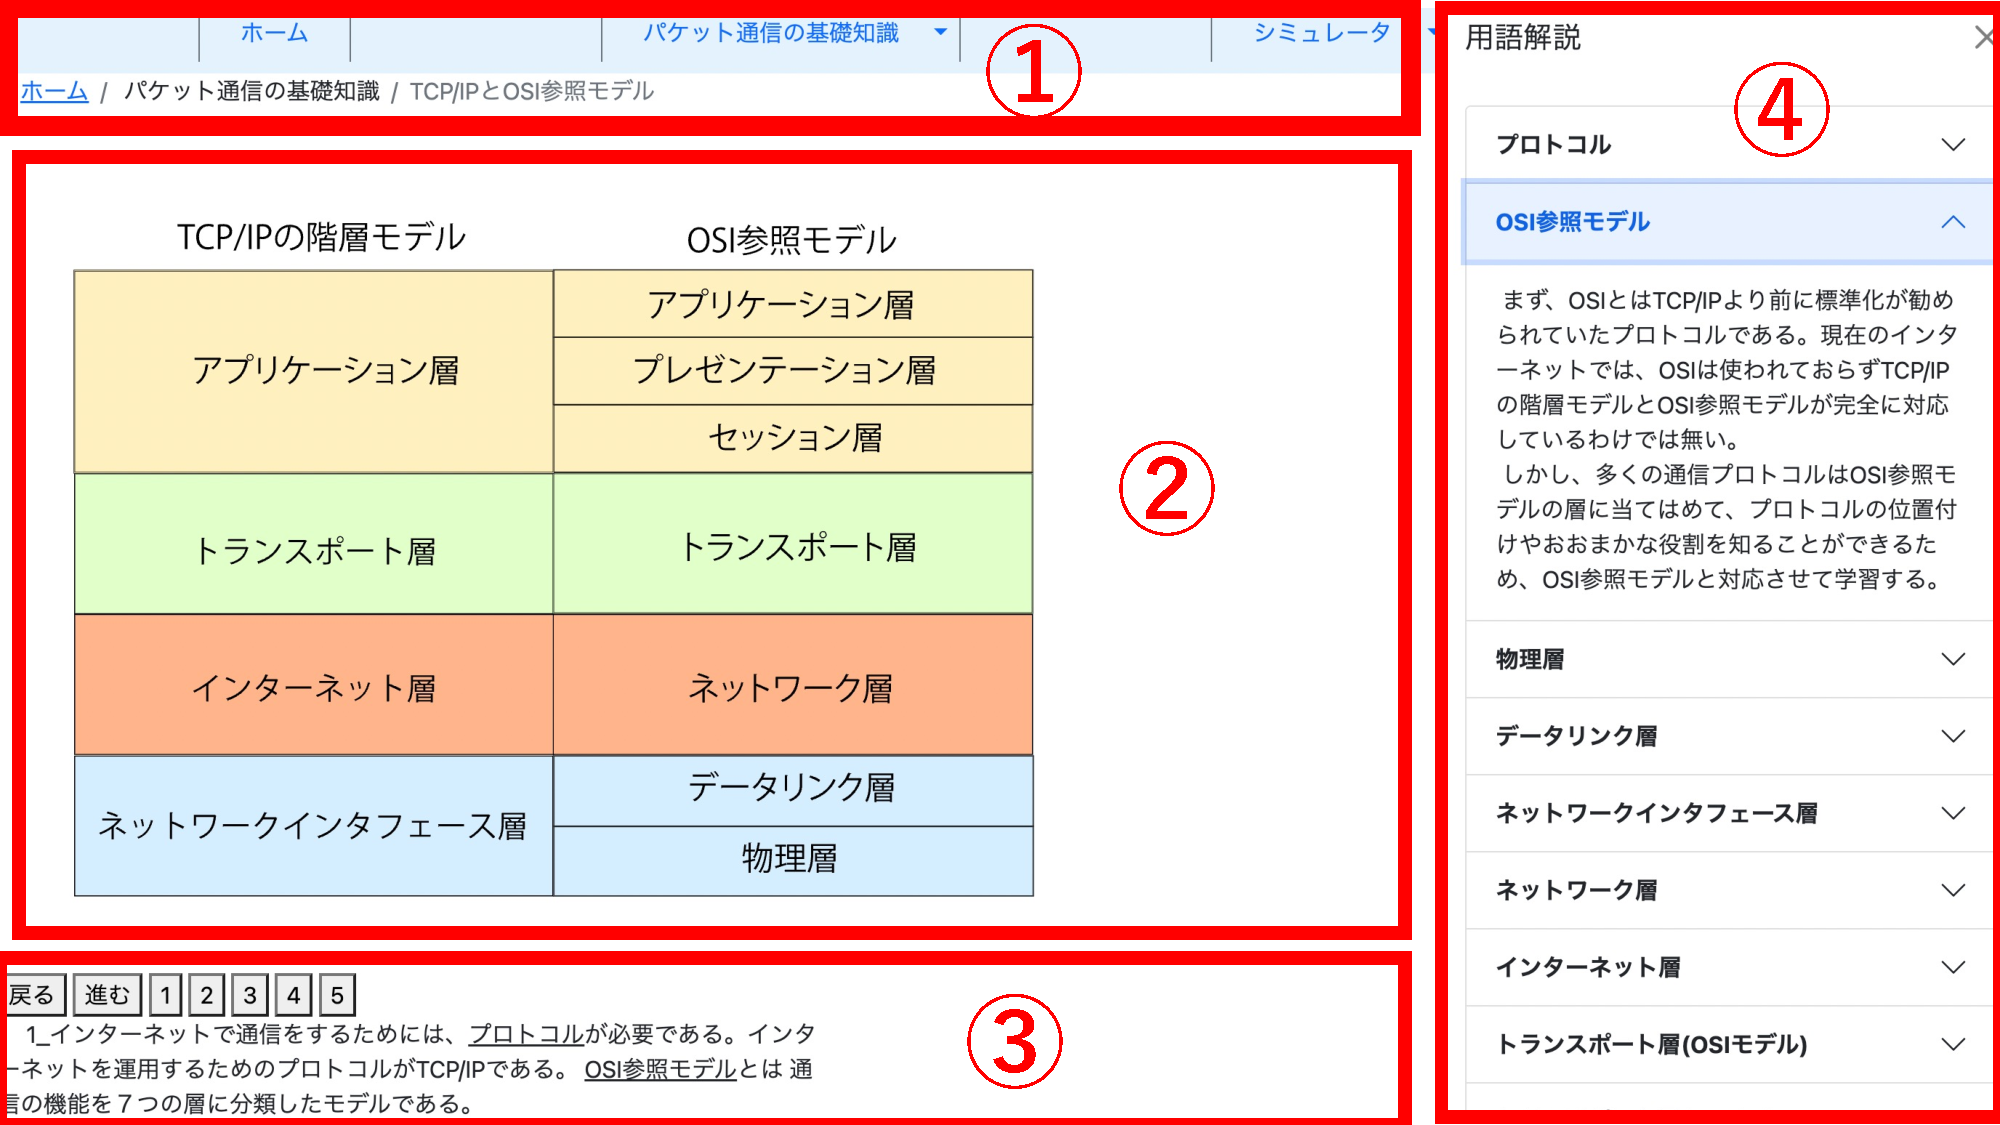
\includegraphics[clip,width=100mm]{figures/gamen.pdf}
\end{center}
 \caption{Web教材の学習画面}
 \label{fig:画面}
\end{figure}

\subsection{ナビゲーション部}
\subsection{メイン表示部}
\subsection{解説表示部}
\subsection{用語解説部}
\subsection{シミュレータ設定部}

\clearpage

\section{教材の実装}%<7章>
a
\subsection{概要}
\subsection{開発に利用した言語}
\subsubsection{HTML}
HTMLとは,Hyper ext Markup Languageの略称であり,ウェブページを作成するために開発された言語である.
\subsubsection{CSS}
\subsubsection{JavaScript}

\subsection{開発に利用したフレームワーク・ライブラリ}
\subsubsection{Bootstrap}
あ

\clearpage

\section{結言}%<8章>
a
%本研究では,ネットワーク通信の基礎を学習する講義形式の授業を補助するWeb教材を開発した.今後このような,生徒や学生が自分で操作し学習できるWeb教材が普及し,講義形式の授業で学習内容を深く理解できるようになることを期待している.
\clearpage

\section{謝辞}%<9章>
本研究の遂行及び本論文の作成にあたり,須田研究室の仲間に多くの手助けを頂きました,深く感謝の意を表します.そして,本論文の作成にあたり多大なる御指導及び御助言を頂きました,須田宇宙准教授に深く感謝の意を表します.
\clearpage

\begin{thebibliography}{99}
%2章
\bibitem{dx_kadai} 総務省: ``令和4年度版 情報通信白書 データ集(第3章第8節)'', 31,
\url{https://www.soumu.go.jp/johotsusintokei/whitepaper/ja/r04/html/nf308000.html#n3802030}, 2022/12/25参照

\bibitem{dx_gaiyou} 経済産業省: ``デジタルガバナンス・コード2.0'', \url{https://www.meti.go.jp/policy/it_policy/investment/dgc/dgc2.pdf}, 2022/12/25参照

%3章
\bibitem{kyoiku_gaiyou} 文部科学省: `` 「教育の情報化に関する手引」(案)第4章 情報教育'', \url{https://www.mext.go.jp/b_menu/shingi/chousa/shotou/056/gijigaiyou/attach/1259396.html}, 2022/12/27参照

\bibitem{syogaku_pro} 文部科学省: `` 小学校プログラミング教育の手引(第三版)'', \url{https://www.mext.go.jp/content/20200218-mxt_jogai02-100003171_002.pdf}, 2022/12/27参照

\bibitem{koukou_sidou} 文部科学省: ``高等学校学習指導要領'', \url{https://www.mext.go.jp/a_menu/shotou/zyouhou/detail/mext_01831.html}, 2022/8/18参照

\bibitem{koukou_kyokasyo} 文部科学省: ``デジタル教科書に関する制度・現状について - 文部科学省'', \url{https://www.mext.go.jp/content/20200710-mxt_kyokasyo-000008653_03.pdf}, 2022/8/25参照
%https://ipsj.ixsq.nii.ac.jp/ej/?action=repository_uri&item_id=195372&file_id=1&file_no=1
\end{thebibliography}

\end{document}
